
\documentclass{article}

% Paquetes plantilla
\usepackage[square, numbers, sort]{natbib}
% \usepackage{cite}
\usepackage{graphicx}
\usepackage[utf8]{inputenc}
\usepackage{amsmath,amssymb,amsfonts}
\usepackage{algorithmic}
\usepackage{textcomp}
\usepackage{subfig}
\usepackage{float}
\usepackage{mathtools}
\usepackage[spanish]{babel}
\usepackage[paper=a4paper,margin=2.75cm]{geometry}
\usepackage{booktabs} % for tables
\usepackage[colorlinks = true,
            linkcolor = blue,
            urlcolor  = blue,
            citecolor = orange,
            anchorcolor = blue]{hyperref} % for hyperlinks
\usepackage{xcolor} % text colors
% Paquetes extra
\usepackage{subcaption, booktabs, siunitx}

\sisetup{
    round-mode          = places, % Rounds numbers
    round-precision     = 2, % to 2 places
}

% Directorio con imagenes
\graphicspath{{./figs/}}

% Cabecera del documento
% ======================================================================

% Titulo
\title{Control de estabilidad de un Péndulo Invertido con Rueda de Reacción}

% Autores
\author{Juan Pablo Sibecas \\ juan.sibecas@gmail.com \\ Control y Sistemas, Facultad de Ingeniería, \\ Universidad Nacional de Cuyo, \\ Mendoza, Argentina}

% Fecha
\date{Julio de 2023}

% Cuerpo del documento
% ======================================================================
\begin{document}

% Comandos definidos por el autor
\renewcommand{\tablename}{Tabla}
% \renewcommand{\color{blue}{#1}}{\azul}

% Crear cabecera
\maketitle

% Resumen
% ======================================================================
\begin{abstract}
    El presente documento presenta los contenidos mínimos que debe tener el proyecto final de la cátedra de Control 
    y Sistemas de la Universidad Nacional de Cuyo. Además, se aclara el estilo de redacción que debe tener el informe 
    del proyecto final y se facilitan algunos recursos para la edición de documentos en \LaTeX.  
\end{abstract}

\begin{table}[h!]
    \begin{center}
        \caption{Descripción de Variables.}
        \label{tab:tabla1}
        \begin{tabular}{l|l}
        \toprule
        \textbf{Símbolo} & \textbf{Descripción}\\
        \midrule
        $\theta$ & Posición angular del péndulo medida en sentido horario desde la posición de equilibrio inestable.\\
        $\varphi$ & Posición angular de la rueda de reacción medida en sentido horario.\\
        $\omega_p$ & Velocidad angular del péndulo.\\
        $\omega_m$ & Velocidad angular de la rueda de reacción.\\

        $J_p$ & Momento de inercia del péndulo respecto a su centro de gravedad.\\
        $J_p^O$ & Momento de inercia del péndulo respecto a la articulación pasiva.\\
        $J_w$ & Momento de inercia de la rueda de reacción respecto a su centro de gravedad.\\
        $m_a$ & Masa del péndulo.\\
        $m_w$ & Masa de la rueda de reacción.\\
        $L_1$ & Distancia del eje pasivo al centro de gravedad del péndulo.\\
        $L_2$ & Longitud del péndulo.\\
        $b_p$ & Coeficiente de fricción en el eje pasivo.\\
        $\tau_m$ & Torque motor aplicado a la rueda de reacción.\\

        $i_a$ & Corriente de armadura del motor.\\
        $V_{in}$ & Tensión de armadura del motor.\\
        $L_a$ & Inductancia del motor.\\
        $R_a$ & Resistencia del motor.\\
        $K_e$ & Constante de FCEM del motor.\\
        $K_t$ & Constante de torque del motor.\\
        $b_m$ & Coeficiente de fricción del motor.\\
        \bottomrule

        \end{tabular}
    \end{center}
\end{table}
\newpage
\section{Introducción}
    \label{sec:intro}
    % En la sección \ref{sec:intro}... 
    El objetivo de este trabajo es lograr la estabilización de un péndulo, en su posición de equilibrio inestable (invertido) mediante el
    accionamiento de una rueda de reacción. Para ello, se propone la utilización de un sistema de control por realimentación de estados,
    utilizando un regulador cuadrático lineal (LQR) para su resolución. Además, se propone el uso de observadores de estado para estimar
    el vector de estados a partir de mediciones parciales de un IMU de 6GDL. \newline

    El péndulo invertido clásico (cart-pole) ha sido estudiado extensivamente por muchos autores en la bibliografía de sistemas de control.
    Una variación del mismo, es el péndulo invertido con rueda de reacción. Este es un sistema mecánico subactuado en cuya base se encuentra 
    una articulación pasiva inmóvil, y en la parte superior del péndulo se acciona una rueda de reacción para inducir variaciones en la cantidad 
    de movimiento angular total del sistema, según su ley de conservación.
    El fenómeno de rueda de reacción es utilizado en muchas aplicaciones de ingeniería, por ejemplo en ingeniería espacial, para la reorientación
    de satélites en órbita.

\section{Desarrollo}
    Como se describió anteriormente, la conservación del momento angular del sistema completo permite la transferencia del mismo entre la rueda de 
    reacción y el brazo del péndulo. La figura \ref{fig:esquema1} muestra el esquema básico de funcionamiento de este fenómeno, donde la variación
    de velocidad de la rueda de reacción induce el movimiento del brazo. El coeficiente de transferencia de velocidades está dado por\cite[text]{1}:
    \begin{equation}
        C = \frac{J_w}{J_p^O + J_w}
    \end{equation}
    %%FALTA CITA AL PAPER DE C
    %%%%%%%%%%%%%%%%%%%%%%
    %%%%%%%%%%%%%%%%%%%%%%%
    %%%%%%%%%%%%%%%%%%%%%%%%
    \begin{figure}[h!]
        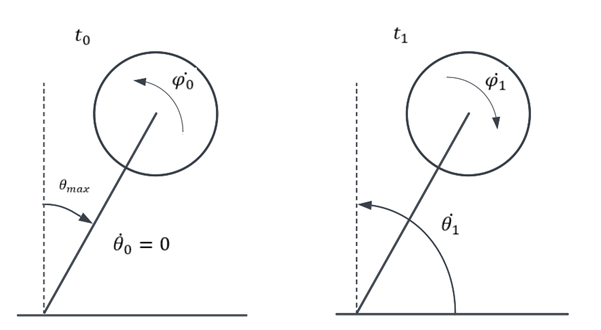
\includegraphics[width=\linewidth]{images/sys_schem.png}
        \caption{Esquema básico.}
        \label{fig:esquema1}
    \end{figure}
    \newpage
    \subsection{Subsistema Mecanico}
        Las ecuaciones que describen el comportamiento mecánico de este sistema se pueden obtener a partir de las ecuaciones de Euler-Lagrange:
        
        
        \begin{equation*}
            \frac{d}{dt}\frac{dL}{d \dot{q_i}} - \frac{dL}{dq_i} = Q_i\\
        \end{equation*}
        Donde $L = T - V$, $q_1 = \theta$ y $q_2 = \varphi$.

        
        La energía cinética $T$ y potencial $V$ del sistema se modelan mediante las siguientes ecuaciones:
        \begin{align*}
            T &= \frac{1}{2} J_p \dot{\theta}^2 + \frac{1}{2} J_w (\dot{\varphi} + \dot{\theta})^2\\
            L &= (m_p L_1 + m_w L_2) g cos(\theta)
        \end{align*}


        \begin{align}
            \ddot{\theta} (J_p^O + J_w) + \ddot{\varphi} J_w - (m_p L_1 + m_w L_2)g \sin(\theta) &= -b_p \dot{\theta}\\
            \ddot{\theta} J_w + \ddot{\varphi} J_w &= \tau_m
        \end{align}

    \subsection{Subsistema eléctrico}
        El modelo del motor de corriente continua está descripto por las siguientes ecuaciones:

        \begin{align}
            V_{in} &= L_a \frac{di_a}{dt} + i_a R_a + \dot{\varphi} K_e\\
            \ddot{\varphi} J_w &= K_t i_a - b_m \dot{\varphi}
        \end{align}

    \section{Representación del Modelo en Espacio de Estados}
    El vector de estados es:
    \begin{equation*}
        x =
        \left[
        \begin{matrix}
            \theta\\
            \omega_p\\
            \omega_m\\
            i_a
        \end{matrix}
        \right]
    \end{equation*}
    La accion de control es 
    $u = V_{in}$ 
    y la salida es 
    $y = \theta$.\newline

    Reemplazando $(4)$ en $(1)$, $\omega_p = \dot{\theta}$, $\omega_m = \dot{\varphi}$, 
    linealizando $\sin(\theta) = \theta$ en $\theta = 0$, 
    y despejando las primeras derivadas de las variables de estado:
    
    \begin{equation*}
        \left[
            \begin{matrix}
                \dot{\theta}\\
                \dot{\omega_p}\\
                \dot{\omega_m}\\
                \dot{i_a}
            \end{matrix}
        \right]
        =
        \left[
        \begin{matrix}
            0           & 1         & 0         & 0\\
            \beta g/m_1   & -b_p/m_1  & b_m/m_1   & -K_t/m_1\\
            0           & 0         & -b_m/J_w  & K_t/J_w\\
            0           & 0         & -K_e/L_a  & -R_a/L_a
        \end{matrix}
        \right]
        \left[
        \begin{matrix}
            \theta\\
            \omega_p\\
            \omega_m\\
            i_a
        \end{matrix}
        \right]
        +
        \left[
        \begin{matrix}
            0\\
            0\\
            0\\
            \frac{1}{L_a}
        \end{matrix}
        \right]
        V_{in}
    \end{equation*}

    \begin{equation*}
        y = 
        \left[
        \begin{matrix}
            1 & 0 & 0 & 0\\
        \end{matrix}
        \right]
        \left[
        \begin{matrix}
            \theta\\
            \omega_p\\
            \omega_m\\
            i_a
        \end{matrix}
        \right]
        = \theta
    \end{equation*}

Donde $\beta = m_p L_1 + m_w L_2$ y $m_1 = J_p^O + J_w$.
\section{Implementación}
Para la simulación del sistema descripto se utilizarán Simulink y MATLAB. Se propone el control del mismo mediante realimentación
de estados, obteniendo la matriz de ganancias de realimentación por un regulador cuadrático lineal(LQR).
\newline
Para la medición de las variables de estado, se propone inicialmente utilizar únicamente un
IMU de 6GDL (Acelerómetro de 3 ejes, Giroscopio de 3 ejes) como inclinómetro, para medir la posición angular del péndulo 
$\theta$ fusionando sensores(filtro de Kalman o complementario). El resto de las variables de estado se estimarán mediante un observador de estado. Si esto no fuera 
suficiente para el control del sistema, se podrán agregar sensores como encoders relativos tanto en el eje activo como pasivo para
obtener mayor información en tiempo real.
\pagebreak
\section{Diagrama de Bloques}
En el siguiente diagrama se muestra la interconexión de los bloques mencionados anteriormente.
\begin{figure}[h!]
    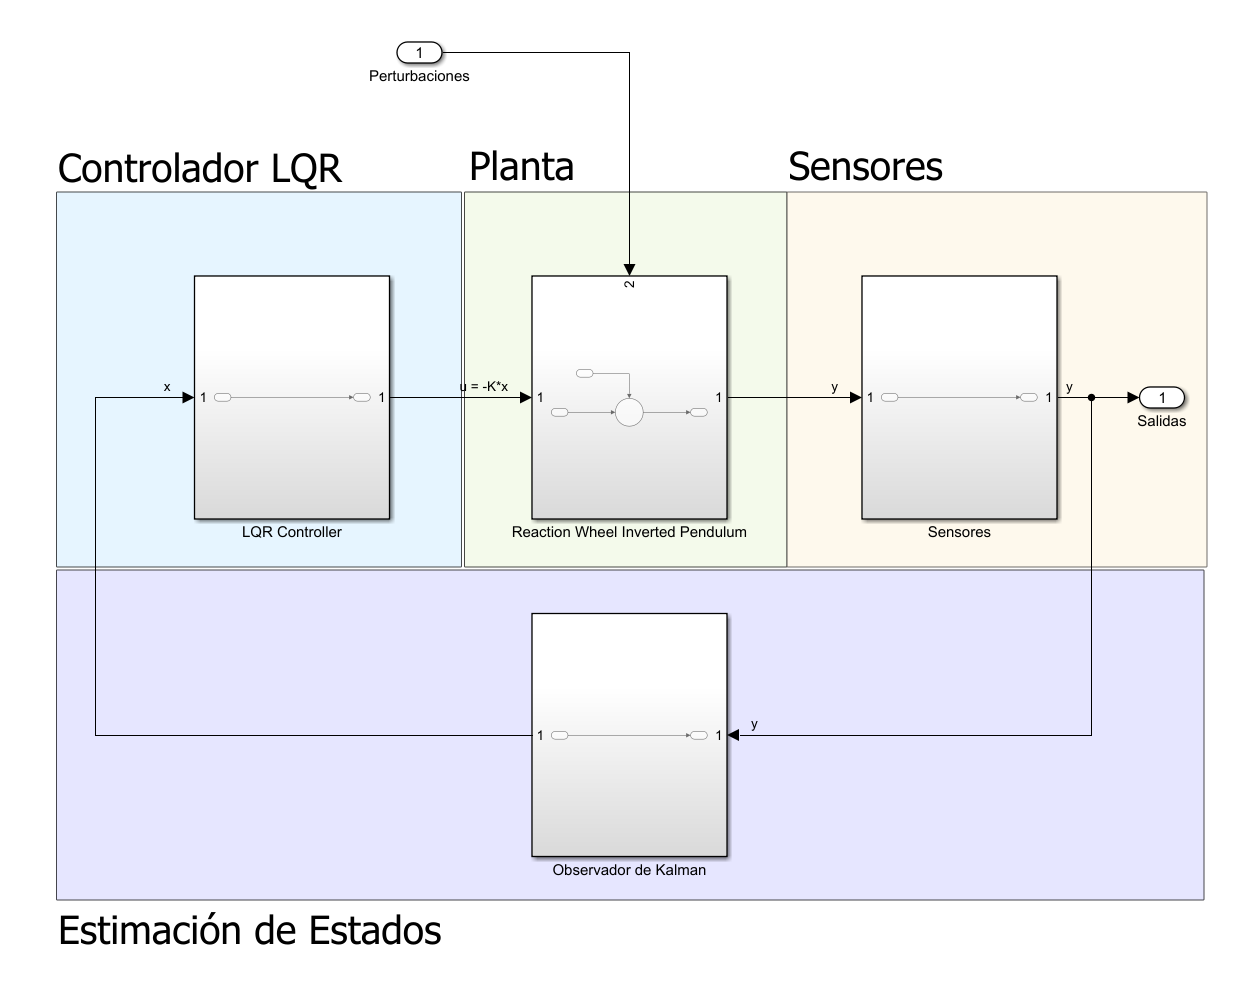
\includegraphics[width=\linewidth]{images/block_diagram.png}
    \caption{Diagrama de bloques.}
    \label{fig:esquema2}
\end{figure}
    

\end{document}